\chapter{2026:Shayan Oveis Gharan}
\normalchapterspacing
\label{chap:gharan}
\begin{center}
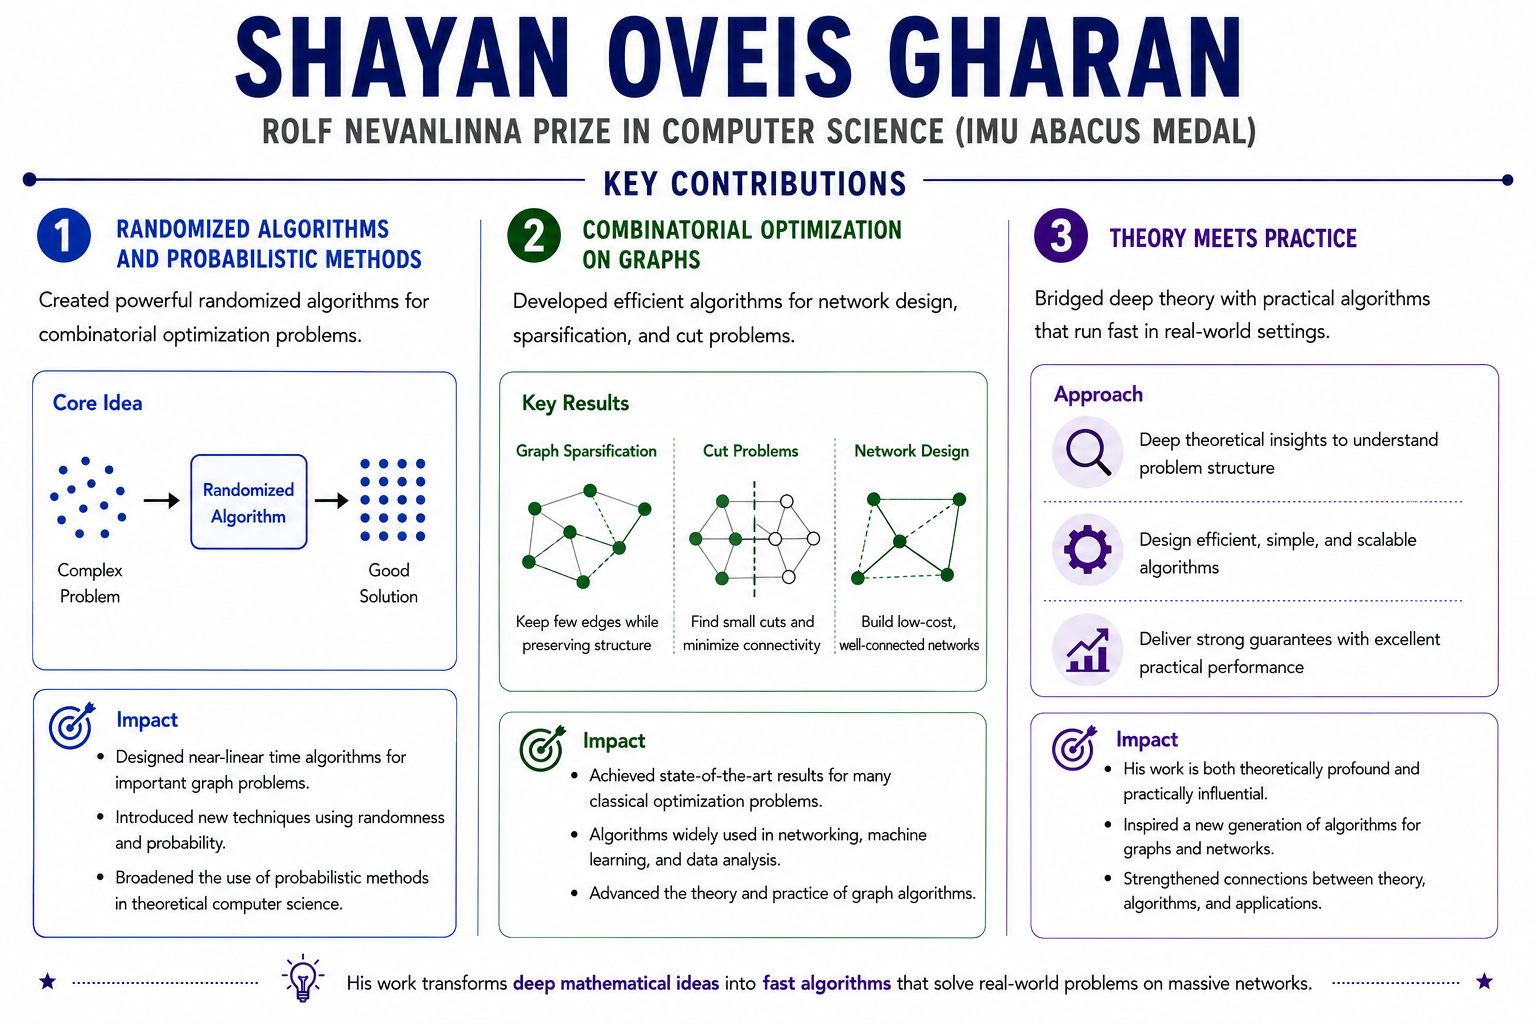
\includegraphics[width=\textwidth]{infographics/abacus12.png}
\end{center}
\index{Oveis Gharan, Shayan}
\booknote{The central habit in this chapter is to encode a combinatorial family as a polynomial, and to read the polynomial's curvature, zeros, and spectra as information about the family.}

\section{An Opening Story: Which Trails Should Stay?}
A small nature reserve has four campsites---north, east, south, and west---joined by five trails forming a square with a diagonal. The rangers must close some trails for maintenance while keeping every campsite reachable from every other. A minimal way to keep the reserve connected is to keep exactly three trails, with none wasted on loops. There are $\binom{5}{3}=10$ ways to choose three of the five trails, but two of those choices form a closed triangle and strand the fourth campsite, leaving $8$ workable choices. Each such choice is a \emph{spanning tree}: three trails that touch all four campsites with no wasted loops.

Now suppose the reserve chooses among the $8$ trees uniformly at random. How likely is each trail to survive? Listing all eight trees answers directly: the diagonal appears in $4$ of them, so it survives with probability $4/8=1/2$; each side trail appears in $5$, so it survives with probability $5/8$. That was easy because the reserve is tiny.

Now add campsites. The complete network on $n$ campsites---every pair directly linked---has $n^{n-2}$ spanning trees: $16$ for $n=4$, about $10^{61}$ (a number with $61$ digits) for $n=40$. The questions ``how many spanning trees?'' and ``how likely is each trail?'' still make sense, but no one will answer them by listing. This is where Oveis Gharan's work begins: the discrete list hides a continuous object---a polynomial---that answers both questions with no listing at all. The 2026 Abacus Medal recognized this habit of reaching for a hidden geometric object when a combinatorial process looks too irregular to control \cite{imu2026}.

\section{The Problem}
Three problems, all phrased as questions a computer must answer without writing out an astronomically large list.

\noindent\textbf{Sampling from a huge family.} Fix a family of combinatorial objects---the spanning trees of a graph, the bases of a matroid, the independent sets of a matroid---and attach a positive weight to every object (for example, the product of weights on its edges). Draw an object at random with probability proportional to its weight. For the four-campsite reserve this is a coin flip among eight trees; for a network of ten thousand sites the family is unimaginably large, yet the answer must come back in seconds.

\noindent\textbf{Approximating the shortest tour.} Given cities with distances obeying the triangle inequality (going directly between two cities is never longer than routing through a third), find the shortest tour that visits every city exactly once. The exact optimum is believed to be computationally hopeless, so the target is a \emph{ratio}: a tour guaranteed to be at most $\alpha$ times the optimum, with $\alpha$ as close to $1$ as possible.

\noindent\textbf{Proving counting inequalities.} Count the independent sets of a matroid by size: $I_k$ independent sets of size $k$. For the uniform matroid on $4$ elements of rank $2$, the counts are $I_0=1$, $I_1=4$, $I_2=6$. Are such sequences always \emph{log-concave}, each term at least the geometric mean of its neighbors, $I_k^2\ge I_{k-1}I_{k+1}$? Mason conjectured a much stronger normalized version in 1978; it stayed open for more than four decades.

All three problems are hard for the same reason: the family is too large to look at, so every argument must summarize the whole family with a smaller object that still remembers the answers.

\section{The World Before}
Before 1976, the travelling salesperson problem had a good heuristic reputation but no provable guarantee. Christofides changed that with an algorithm that is almost ridiculously short to describe, and whose $3/2$ approximation ratio then resisted improvement for roughly forty-five years \cite{christofides76}.

\noindent\textbf{Christofides' architecture.} First build a minimum spanning tree: connect all cities with the cheapest possible set of roads. This costs at most the length of an optimal tour, because deleting one road from any tour leaves a spanning tree. Second, look at the vertices where the tree has an odd number of incident edges---they cannot close into a valid tour yet---and add a minimum-weight perfect matching among exactly those vertices. That matching costs at most half an optimal tour, because an optimal tour, restricted to the odd vertices, splits into two matchings of total length at most the tour. Third, \emph{shortcut}: walk along the tree and the matching and, whenever the walk revisits a city, jump over it. The triangle inequality guarantees that shortcuts never lengthen the tour. Total: $1+\tfrac12=\tfrac32$ times optimal.

\noindent\textbf{Why $3/2$ survived.} The proof is tight: there are instances where the tree alone costs a whole tour and the matching is forced to cost half a tour at the same time. Every improvement attempt used the same division of labor---one argument pays for connectivity, a separate argument pays for parity repair---and each layer kept paying the same bill. After decades it became clear that any real improvement must break the coupling: it must choose a spanning tree whose random choices are correlated with the parity repair that will follow. That requires a distribution over trees with very specific statistical properties, which is exactly what nobody had.

\noindent\textbf{Markov chains, one family at a time.} To sample from a huge family, a standard tool is a \emph{Markov chain}: start with any object, make small random changes (drop an edge, add an edge), and hope the walk quickly forgets where it started. The obstacle is proving \emph{rapid mixing}. Before the work in this chapter, mixing proofs were done family by family with ad hoc tools---conductance arguments that hunt for a bottleneck, couplings that pair two walks and show they meet. Each success looked different, and there was no common certificate a newcomer could reuse.

\noindent\textbf{Log-concavity sat in convex geometry.} Log-concave sequences and functions had a rich life in convex geometry and probability---Brunn--Minkowski theory, Alexandrov--Fenchel inequalities, the geometry of polytopes---but almost nobody connected them to algorithms. Mason's 1978 conjecture about the normalized counts $I_k/\binom nk$ sat exactly at this intersection: clearly combinatorial, provable by no combinatorial tool known then.

\section{The New Idea}
The unifying move is to change the type of the object being studied. A family of discrete objects becomes a single polynomial, and the polynomial's geometry---where it is concave, where its zeros live, what its spectrum is---becomes a certificate that algorithms can consume. Four named ideas form the toolkit.

\subsection{A family becomes a polynomial}
For a graph $G$ with an edge variable $z_e$ per edge, define the \emph{spanning-tree polynomial}
\[
T_G(z)=\sum_{\mathcal{T}\text{ spanning tree}}\;\prod_{e\in\mathcal{T}} z_e,
\]
one monomial per tree. The polynomial is a storage device: the coefficient of a monomial counts the trees containing that set of edges. More importantly, derivatives are exactly the operations an algorithm needs. Setting $z_e=0$ \emph{forbids} edge $e$; differentiating with respect to $z_e$ \emph{forces} it. The ratio $z_e\,\partial_{z_e}\log T_G$, evaluated at $z_e=1$, is the probability that a uniformly random spanning tree contains edge $e$. A combinatorial question about a huge family has become a calculus question about one object.

\subsection{Log-concavity and negative dependence}
A positive polynomial $p$ is \emph{log-concave} on the positive orthant when $\log p$ bends downward in every direction there. The word is geometry, but it can support useful statistical consequences: in the strongly log-concave and matroid settings relevant here, it underlies mixing results and known negative-dependence consequences. Plain log-concavity alone is not equivalent to negative dependence. The stronger hypotheses also survive the operations an algorithm needs: conditioning (take a derivative) and restriction (set variables to zero). A proof that the relevant polynomial is strongly log-concave is therefore a promise that the whole sequence of conditional distributions the algorithm creates will stay well behaved.

\emph{Stable polynomials} are the mechanism that produces log-concavity. A multivariate polynomial is stable when it has no zeros with all variables in the upper half-plane; this is the natural generalization of a one-variable polynomial with all real roots. Real-rootedness was already known to force log-concavity of coefficient sequences, and stability inherits that power in many variables while being closed under exactly the operations---differentiation, specialization, limits---that a proof needs.

\subsection{Spectral independence: a local certificate}
For a distribution on subsets, define the \emph{influence} of one element on another: how much does conditioning on one element being present change the marginal probability of another? A large influence entry is a suspicion of a bottleneck; a large \emph{eigenvalue} of the influence matrix is the real disease, because a matrix can have small entries yet greatly amplify a well-chosen direction. \emph{Spectral independence} requires the largest eigenvalue of every influence matrix---under \emph{every} partial assignment the chain might encounter---to stay bounded. This converts ``prove there is no hidden bottleneck'' into ``bound the eigenvalues of some small matrices,'' and it is exactly the local certificate a fast-mixing proof needs.

\subsection{Entropic rounding: how $3/2$ fell}
The last idea closes the TSP story. Solve a fractional relaxation of the tour problem: a point $x$ in a polytope that mixes connectivity and parity information and costs at most the optimal tour. Then round it to a real tour. The old rounding rules chose edges independently and paid the same parity bill every time. The new rule is \emph{entropic rounding}: choose the distribution over spanning trees with maximum entropy among all distributions whose marginals match $x$, then sample from it. Because the tree polynomial has the required stability and correlation properties, the sampled tree is globally correlated in exactly the way the parity repair needs, and the two bills---connectivity and parity---can no longer both be maximally expensive at once. The result: approximation ratio $3/2-\eps$ for a fixed constant $\eps>10^{-36}$ \cite{karlin-tsp}, the first improvement over Christofides in nearly half a century.

The conceptual shift, in one line: \emph{a family of trees can be a determinant; a distribution can be a polynomial; correlations can be an operator; a mixing proof can be a curvature argument.}

\section{How It Works: Worked Examples}
\subsection{The triangle: three trees, one polynomial}
Take the triangle on vertices $\{1,2,3\}$ with edge weights $a$ (between $1$ and $2$), $b$ (between $2$ and $3$), and $c$ (between $1$ and $3$). Every spanning tree omits exactly one edge, so the spanning-tree polynomial is
\[
T(a,b,c)=ab+ac+bc.
\]
Set $a=b=c=1$. Then $T=3$: the triangle has three spanning trees. Edge $a$ appears in the trees $\{ab,ac\}$, two out of three, so a uniformly random tree contains edge $a$ with probability $2/3$.

Now the polynomial answers the same question by calculus. The derivative
\[
a\,\frac{\partial T}{\partial a}=a(b+c)=1\cdot(1+1)=2
\]
counts, with weight, the trees containing edge $a$; dividing by $T=3$ gives $2/3$. Equivalently, the \emph{logarithmic derivative}
\[
a\,\frac{\partial}{\partial a}\log T=\frac{a(b+c)}{ab+ac+bc}=\frac{2}{3}
\]
is the marginal probability. \emph{A derivative that looks analytic is a probability.}

\subsection{A resistor agrees}
Now treat each edge as a $1$-ohm resistor and compute the \emph{effective resistance} between the endpoints of edge $a$: the resistance of the whole network seen from those two terminals. The route through $b$ and $c$ in series has resistance $1+1=2$ ohms; the direct edge $a$ is a $1$-ohm path in parallel with it, so
\[
R_{\mathrm{eff}}=\frac{1\cdot 2}{1+2}=\frac{2}{3}\ \text{ohms}.
\]
The electrical identity behind random spanning trees (Kirchhoff) says: the probability that an edge belongs to the random tree equals its conductance times the effective resistance between its endpoints. The conductance is $1$, so the probability is $2/3$ again. Two computations that look completely different---counting trees, and reducing resistor networks---deliver the same number. That coincidence is the pattern: \emph{write the partition function, differentiate it, read the derivative as a marginal, and recognize the marginal as a physical quantity.}

The identity is not a special case of equal weights. Try $a=1$, $b=2$, $c=3$: the polynomial gives $T=11$ and probability $a(b+c)/T=5/11$. The series path $b,c$ has resistance $1/2+1/3=5/6$; in parallel with the $1$-ohm edge,
\[
R_{\mathrm{eff}}=\frac{1}{1+6/5}=\frac{5}{11},
\]
and conductance times resistance is $5/11$ again.

\subsection{Mason's conjecture on a small matroid}
A sequence $x_0,x_1,\ldots$ is \emph{log-concave} when $x_k^2\ge x_{k-1}x_{k+1}$ for every $k$: each term is at least the geometric mean of its neighbors. The binomial coefficients $\binom 4k=1,4,6,4,1$ are log-concave, since $4^2=16\ge 1\cdot 6=6$ and $6^2=36\ge 4\cdot 4=16$.

The uniform matroid $U_{2,4}$ keeps every subset of $\{1,2,3,4\}$ of size at most $2$ independent. Its counts are $I_0=1$, $I_1=4$, $I_2=6$---the entries of the binomial row, by design. Mason's conjecture (now a theorem of Anari, Liu, Oveis Gharan, and Vinzant \cite{anari20}) says the \emph{normalized} counts are log-concave:
\[
\left(\frac{I_k}{\binom nk}\right)^2\ge \frac{I_{k-1}}{\binom n{k-1}}\cdot\frac{I_{k+1}}{\binom n{k+1}},
\]
where $n$ is the number of elements of the matroid---for $U_{2,4}$, $n=4$. (Do not normalize by the rank $\binom rk$; the ground-set size $n$ is the right denominator.) Clearing denominators gives the working form
\[
I_k^2\ge I_{k-1}\,I_{k+1}\,\frac{(k+1)(n-k+1)}{k(n-k)}.
\]
Check $k=1$ for $U_{2,4}$:
\[
I_1^2=16,\qquad I_0\,I_2\,\frac{2\cdot 4}{1\cdot 3}=1\cdot 6\cdot\frac{8}{3}=16.
\]
Equality---the uniform matroid is the perfectly balanced case, exactly where the bound is sharp.

The conjecture is meaningful for matroids that are not uniform. Take the graphic matroid of the complete graph $K_4$: its elements are the $6$ edges, and independent sets are forests. The counts are $I_0=1$, $I_1=6$, $I_2=15$ (any two edges), $I_3=16$ (the spanning trees, by Cayley's formula $n^{n-2}=16$), and $I_4=0$. Here $n=6$, and the $k=2$ check reads
\[
I_2^2=225,\qquad I_1\,I_3\,\frac{(3)(5)}{(2)(4)}=6\cdot 16\cdot\frac{15}{8}=180,
\]
and $225\ge 180$ holds. The plain sequence $1,6,15,16$ is log-concave too ($15^2=225\ge 6\cdot 16=96$), but the normalized inequality is strictly stronger, and it is the strong form that powers the algorithms: it is exactly the statement that the independence polynomial is log-concave in the sense needed for fast sampling.

\section{The Mathematics in Brief}
\emph{The spanning-tree polynomial is a determinant.} The matrix-tree theorem: form the weighted Laplacian $L$ with diagonal entries equal to the sum of the edge weights incident to a vertex and off-diagonal entries $-w_{uv}$; delete any one row and column; the determinant is exactly $T_G(z)$. Determinants are more than a computation trick: they give the polynomial a spectral life, including its stability, that pure combinatorics cannot see.

\emph{Log-concavity is a statement about covariance.} For a positive polynomial $p$, the Hessian
\[
\nabla^2\log p=\frac{p\,\nabla^2p-(\nabla p)(\nabla p)^{\mathsf T}}{p^2}
\]
is negative semidefinite exactly when $p$ is log-concave. The first derivatives of $\log p$ are marginal probabilities; the second derivatives, after subtracting products of first derivatives, are conditional covariances. Negative semidefiniteness says these covariances are nonpositive in every direction: negative dependence, uniformly. The ``why'': the numerator is a covariance-like object in disguise, and concavity forbids any direction in which including one element systematically amplifies another.

\emph{Influence matrices.} For a distribution on binary variables and a partial assignment $\tau$, define
\[
\Psi^\tau_{ij}=\PP(X_j=1\mid X_i=1,\tau)-\PP(X_j=1\mid X_i=0,\tau).
\]
Spectral independence requires $\lambda_{\max}(\Psi^\tau)\le C$ for every $\tau$. The eigenvalue, not the entries, is the right measure: the all-ones matrix has every entry $1$ but operator norm $m$, and a chain that must navigate such a collective push needs to know about it.

\emph{Local certificates, global mixing.} The payoff theorem (Asadi, Oveis Gharan, and Saberi \cite{asadi20}; sharpened by Anari, Liu, Oveis Gharan, and Vinzant \cite{anari21}) applies under specific strong log-concavity, spectral-independence, and chain hypotheses; plain log-concavity by itself is not a universal mixing theorem. Under those hypotheses, the relevant local chain mixes rapidly. Sampling then becomes a usable subroutine, and counting rides on it: a telescoping product of partition-function ratios, each factor estimated from samples at a nearby parameter, yields a fully polynomial randomized approximation scheme for counting matroid bases \cite{anari19}.

\emph{The TSP, in two layers.} The subtour-elimination linear program relaxes tours to fractional vectors $x_e$ on edges, costing at most the optimum tour. The rounding layer chooses a distribution over spanning trees whose marginals match $x$ and which has maximum entropy among all such distributions; the relevant stability and strong log-concavity properties of $T_G$ supply the correlation control that keeps the parity-repair bill in check. The layers are inseparable: a relaxation that sees structure is useless without a rounding rule that respects it.

\section{Limits and Modern Views}
The certificate-based picture has boundaries worth knowing before they bite.

\noindent\textbf{Certificates can be hard to verify.} A polynomial may be log-concave or stable, but checking that property computationally is not free, and a theorem about an inaccessible certificate does not by itself produce an algorithm.

\noindent\textbf{Chain steps can be expensive.} Fast mixing is measured in number of steps; the steps themselves must be cheap, and a local move over a huge family may involve a determinant or a linear-system solve per step. The true running time is steps times per-step cost.

\noindent\textbf{Constants hide in guarantees.} The metric TSP improvement is $3/2-\eps$ for a fixed constant $\eps>10^{-36}$ \cite{karlin-tsp}---a genuine theoretical milestone that does not change the number on a real logistics invoice. Approximation theory measures ratios asymptotically; practice measures constants.

\noindent\textbf{Log-concavity fails at phase transitions.} Real systems have regimes---high density, sharp thresholds---where the balanced, negatively dependent world breaks down and bottlenecks reappear. The certificates are true only where their hypotheses hold, and knowing where they fail is part of using them.

The field moved outward from these boundaries. The geometry-of-polynomials program now touches approximate counting, high-dimensional statistical physics, convex geometry, and algebraic combinatorics via Hodge theory; spectral independence has become a standard tool for spin systems and other Gibbs distributions; entropic rounding opened a research line on correlation-aware rounding beyond TSP. Open directions include weaker stability notions that still imply negative dependence, adaptive and nonreversible chain designs, and approximate or learned certificates. The habit of this chapter---encode, then read geometry---survives every one of these changes.

\section{Exercises and Self-Study Guide}
\begin{enumerate}[label=\textbf{E\arabic*.}]
\item List all spanning trees of a path on four vertices and write its weighted spanning-tree polynomial.
\hint{A spanning tree of a four-vertex graph has three edges, and the path has exactly three. There is exactly one tree; the polynomial is a single monomial, and every edge marginal is $1$. Compare with the triangle, where every tree omits one edge.}
\item For the triangle with weights $a=1$, $b=2$, $c=3$, compute the probability that a random weighted tree contains edge $a$, in two ways: from the polynomial $T=ab+ac+bc$, and from the series--parallel effective resistance between the endpoints.
\hint{Both give $5/11$: the series path $b,c$ has resistance $1/2+1/3=5/6$, and in parallel with the $1$-ohm edge the effective resistance is $1/(1+6/5)=5/11$.}
\item Verify Mason's inequality $I_k^2\ge I_{k-1}I_{k+1}(k+1)(n-k+1)/\bigl(k(n-k)\bigr)$ for $U_{2,4}$ at $k=1$ and for the graphic matroid of $K_4$ at $k=2$.
\hint{Use $n=4$ for $U_{2,4}$ and $n=6$ for $K_4$ (the number of edges, not the rank $3$). The counts are $1,4,6$ and $1,6,15,16$; the two checks are equality and $225\ge 180$.}
\item Build the two-state Markov chain with transition matrix $\begin{pmatrix}1-a&a\\b&1-b\end{pmatrix}$. Find its stationary distribution and eigenvalues, and decide when mixing is fast.
\hint{The stationary distribution is proportional to $(b,a)$; the eigenvalues are $1$ and $1-a-b$, so the spectral gap $a+b$ controls the mixing speed.}
\item Give a matrix whose every entry is small but whose operator norm is large.
\hint{The all-ones matrix $J$ has $\norm{J}=m$ while every entry is $1$: the vector $(1,\ldots,1)$ is an eigenvector with eigenvalue $m$. Small entries can still push collectively.}
\item Design a local Markov chain for sampling independent sets of a small graph, and identify a likely bottleneck.
\hint{Use Glauber dynamics: add or delete a vertex while maintaining independence. On a star graph the chain must cross between ``center chosen'' and ``center absent''; thin cuts between such regions control the mixing time.}
\item Compute the total variation distance between the distributions $\mu=(0.9,0.1)$ and $\nu=(0.7,0.3)$ on $\{0,1\}$, and explain what the number means.
\hint{$\norm{\mu-\nu}_{\mathrm{TV}}=\frac12\sum_x\abs{\mu(x)-\nu(x)}=\frac12(0.2+0.2)=0.2$; it is the largest probability gap any event can detect.}
\end{enumerate}

\booknote{A final exercise in judgment: whenever a polynomial makes a combinatorial theorem easy, ask what the polynomial made invisible. It answers questions about marginals, correlations, and counts instantly; it does not show you any single object. Decide, for one of your own problems, whether the algorithm needs a specific object or only its statistics---and if it needs the object, find the way back out.}
\clearpage
